\section{Opis Modelu SI}\label{sec:opis-modelu-si}

Model sztucznej inteligencji został zaprojektowany w celu klasyfikacji zdjęć kości k8 (ośmiościennych) do jednej z ośmiu klas, odpowiadających cyfrom od 1 do 8 na każdej ze ścianek.
Do implementacji modelu wykorzystano moduły scikit-learn oraz wchodzący w jego skład Keras, obecnie jako część modułu Tensorflow, który umożliwia łatwe tworzenie i trenowanie sieci neuronowych.
\textit{Biblioteka Keras jest wygodnym opakowaniem (wrapperem) dla modeli DL używanych do oszacowań klasyfikacji lub regresji]} [Donald J. Norris, 2020 s. 355 wydanie APN PROMISE SA]

--- TODO --- \\
cytowanie dodać do bibtex

\subsection{Przygotowanie danych}\label{subsec:przygotowanie-danych}

Dane wejściowe zostały podzielone na zestawy treningowy i walidacyjny w proporcji 70:30.
W celu zwiększenia różnorodności danych treningowych zastosowano techniki augmentacji obrazów dostępne w klasie ImageDataGenerator, takie jak:

\begin{itemize}
    \item obrót o losowy kąt w zakresie do 90°,
    \item przesunięcia poziome i pionowe,
    \item transformacje perspektywiczne (shear) ,
    \item losowe powiększenia (zoom) .
\end{itemize}

W szczególności należy zaznaczyć, że finalnie uniknięto początkowo przeoczonego błędu,
jakim jest tworzenie obrazów lustrzanych w wyżej wymienionych transformacjach, gdyż obrazy lustrzane
sprawiały że ścianki 2 oraz 5 były znacznie gorzej rozróżnialne przez wytrenowany model.

% TODO - check czy quote na ściankach się kompiluje

\subsection{Architektura modelu}\label{subsec:architektura-modelu}

Model jest wielowarstwową siecią konwolucyjną (CNN) składającą się z następujących elementów:

\begin{itemize}
    \item Warstwy wejściowej w rozmiarze 64 na 64 piksele, ale o jednym kanale (skala szarości)
    \item Trzech warstw konwolucyjnych z funkcją aktywacji ReLU:
    \item Warstwy spłaszczającej (Flatten),
    \item Dwóch w pełni połączonych warstw (Dense), z których pierwsza również używa aktywacji ReLu,
a ostatnia używa funkcji aktywacji softmax do klasyfikacji na 8 klas.
\end{itemize}

W przypadku zmiany kości na taką z inną ilością ścianek, np. na również rozważane kości k4, k6, albo k16,
ostatnia warstwa musiałaby również ulec odpowiedniej zmianie, tak aby ilość neuronów odpowiadała ilości ścianek na używanej kości.

\subsection{Trenowanie modelu}\label{subsec:trenowanie-modelu}

Model został skompilowany z wykorzystaniem optymalizatora Adam,
funkcji strat sparse categorical crossentropy dostępnej w module tensorflow oraz metryki dokładności.
Proces trenowania obejmował 20 epok:

\begin{verbatim}
model.compile(
    optimizer='adam',
    loss='sparse_categorical_crossentropy',
    metrics=['accuracy']
)
history = model.fit(
    train_data,
    validation_data=val_data,
    epochs=20,
    steps_per_epoch=train_data.samples,
    validation_steps=val_data.samples
)
\end{verbatim}

\subsection{Wyniki}\label{subsec:wyniki}

Podczas trenowania osiągnięto następujące końcowe wyniki:

\begin{itemize}
    \item Dokładność na zbiorze treningowym: 0,9375 \texttt{final\_train\_acc},
    \item Dokładność na zbiorze walidacyjnym: 1,0  \texttt{final\_val\_acc},
    \item Strata na zbiorze treningowym: 0,0786  \texttt{final\_train\_loss},
    \item Strata na zbiorze walidacyjnym: 0,0274  \texttt{final\_val\_loss}.
\end{itemize}

Wyniki zostały również zwizualizowane na wykresach przedstawiających zmianę dokładności i straty w trakcie trenowania.

\begin{figure}[H]
    \centering
    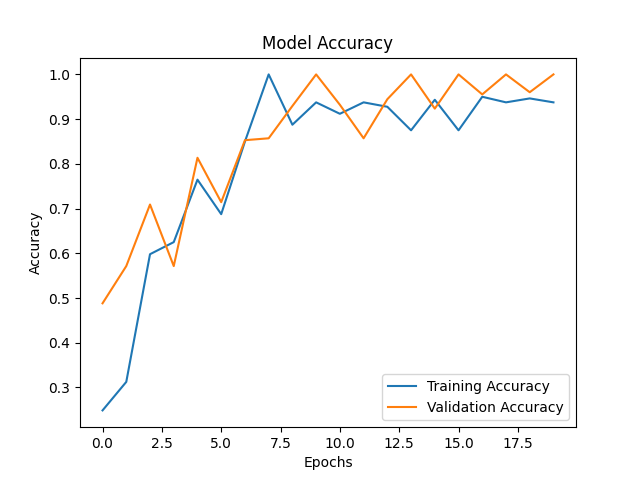
\includegraphics[width=0.7\textwidth]{chapters/04-czytanie/figures/ModelAcc1}
    \caption{Wykres dokładności modelu.}
    \label{fig:ModelAcc}
\end{figure}

\begin{figure}[H]
    \centering
    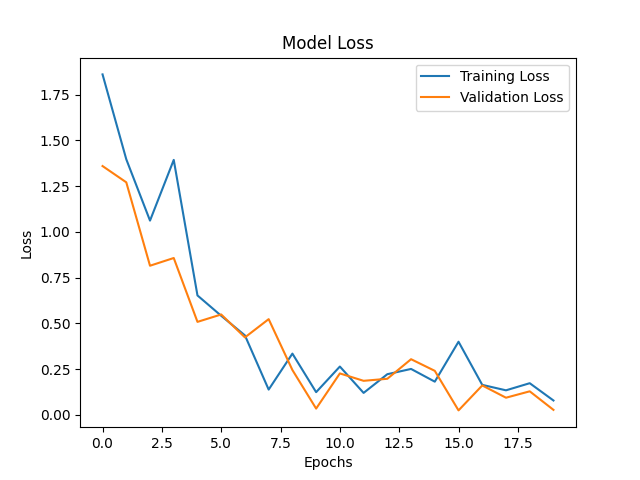
\includegraphics[width=0.7\textwidth]{chapters/04-czytanie/figures/ModelLoss1}
    \caption{Wykres straty modelu.}
    \label{fig:ModelLoss}
\end{figure}

Model został zapisany w formacie \texttt{keras} i jest gotowy do użycia w systemie rozpoznawania liczb na ośmiościennej kości,
opisanym w kolejnej sekcji.

